
% ============================================================================

\section{Avaliação de desempenho e escalabilidade}
\label{sec:desempenho}

A avaliação de desempenho do pipeline apoiou-se em métricas reais coletadas de
duas fontes complementares: (i) os arquivos de \textit{benchmark} gerados
automaticamente pela diretiva \texttt{benchmark} do Snakemake, um por regra,
contendo o tempo de relógio (\textit{wall-clock}), o tempo de CPU e o pico de
memória residente (\texttt{max\_rss}); e (ii) as estatísticas de execução do
GATE (\texttt{stat-*.txt}), que reportam o número de partículas primárias
simuladas e a taxa de processamento (\textit{primaries per second}, pps). As
medições foram conduzidas em duas plataformas: uma estação local equipada com
processador Intel Core i5--1335U (10 núcleos, 12 \textit{threads}) e o servidor
de alto desempenho (HPC) com dois processadores Intel Xeon Gold 5318Y
(48 núcleos físicos, 96 lógicos) e 503~GB de RAM.

\subsection{Perfil de tempo por etapa do pipeline}
\label{sec:perfil}

A Tabela~\ref{tab:benchmarks} consolida o desempenho de cada etapa para a
amostra representativa \texttt{0801\_clean\_fdk\_256}, medido na máquina local.

\begin{table}[htbp]
\centering
\caption{Desempenho por etapa do pipeline (máquina local, i5--1335U).}
\label{tab:benchmarks}
\begin{tabular}{lrrrr}
\toprule
\textbf{Etapa} & \textbf{Wall (s)} & \textbf{CPU (s)} & \textbf{RAM pico (MB)} & \textbf{\% total} \\
\midrule
Simulação Monte Carlo (GATE) & 211,15 & 194,05 & 2.417,8 & 81,4 \\
Segmentação (TotalSegmentator) & 38,39 & 13,90 & 5.179,6 & 14,8 \\
Cálculo de doses (DVH) & 7,64 & 7,42 & 537,2 & 2,9 \\
Conversão NPY$\rightarrow$NIfTI & 1,23 & 0,90 & 241,5 & 0,5 \\
Conversão NPY$\rightarrow$MHD & 0,64 & 0,44 & 281,9 & 0,2 \\
Consolidação (soma de doses) & 0,44 & 0,00 & 3,1 & 0,2 \\
\midrule
\textbf{Total} & \textbf{259,48} & --- & --- & \textbf{100,0} \\
\bottomrule
\end{tabular}
\end{table}

A Figura~\ref{fig:perfil} apresenta essa distribuição.
Observa-se que a simulação Monte Carlo concentra \textbf{81,4\%} do tempo total
de execução, enquanto as cinco etapas restantes somadas respondem por apenas
48,3~s (18,6\%). Essa concentração caracteriza a simulação como o único gargalo
computacional relevante: o desempenho global do fluxo de trabalho é governado
quase integralmente por essa etapa, de modo que a variação das demais entre
diferentes plataformas é desprezível para o tempo total.

\begin{figure}[htbp]
\centering
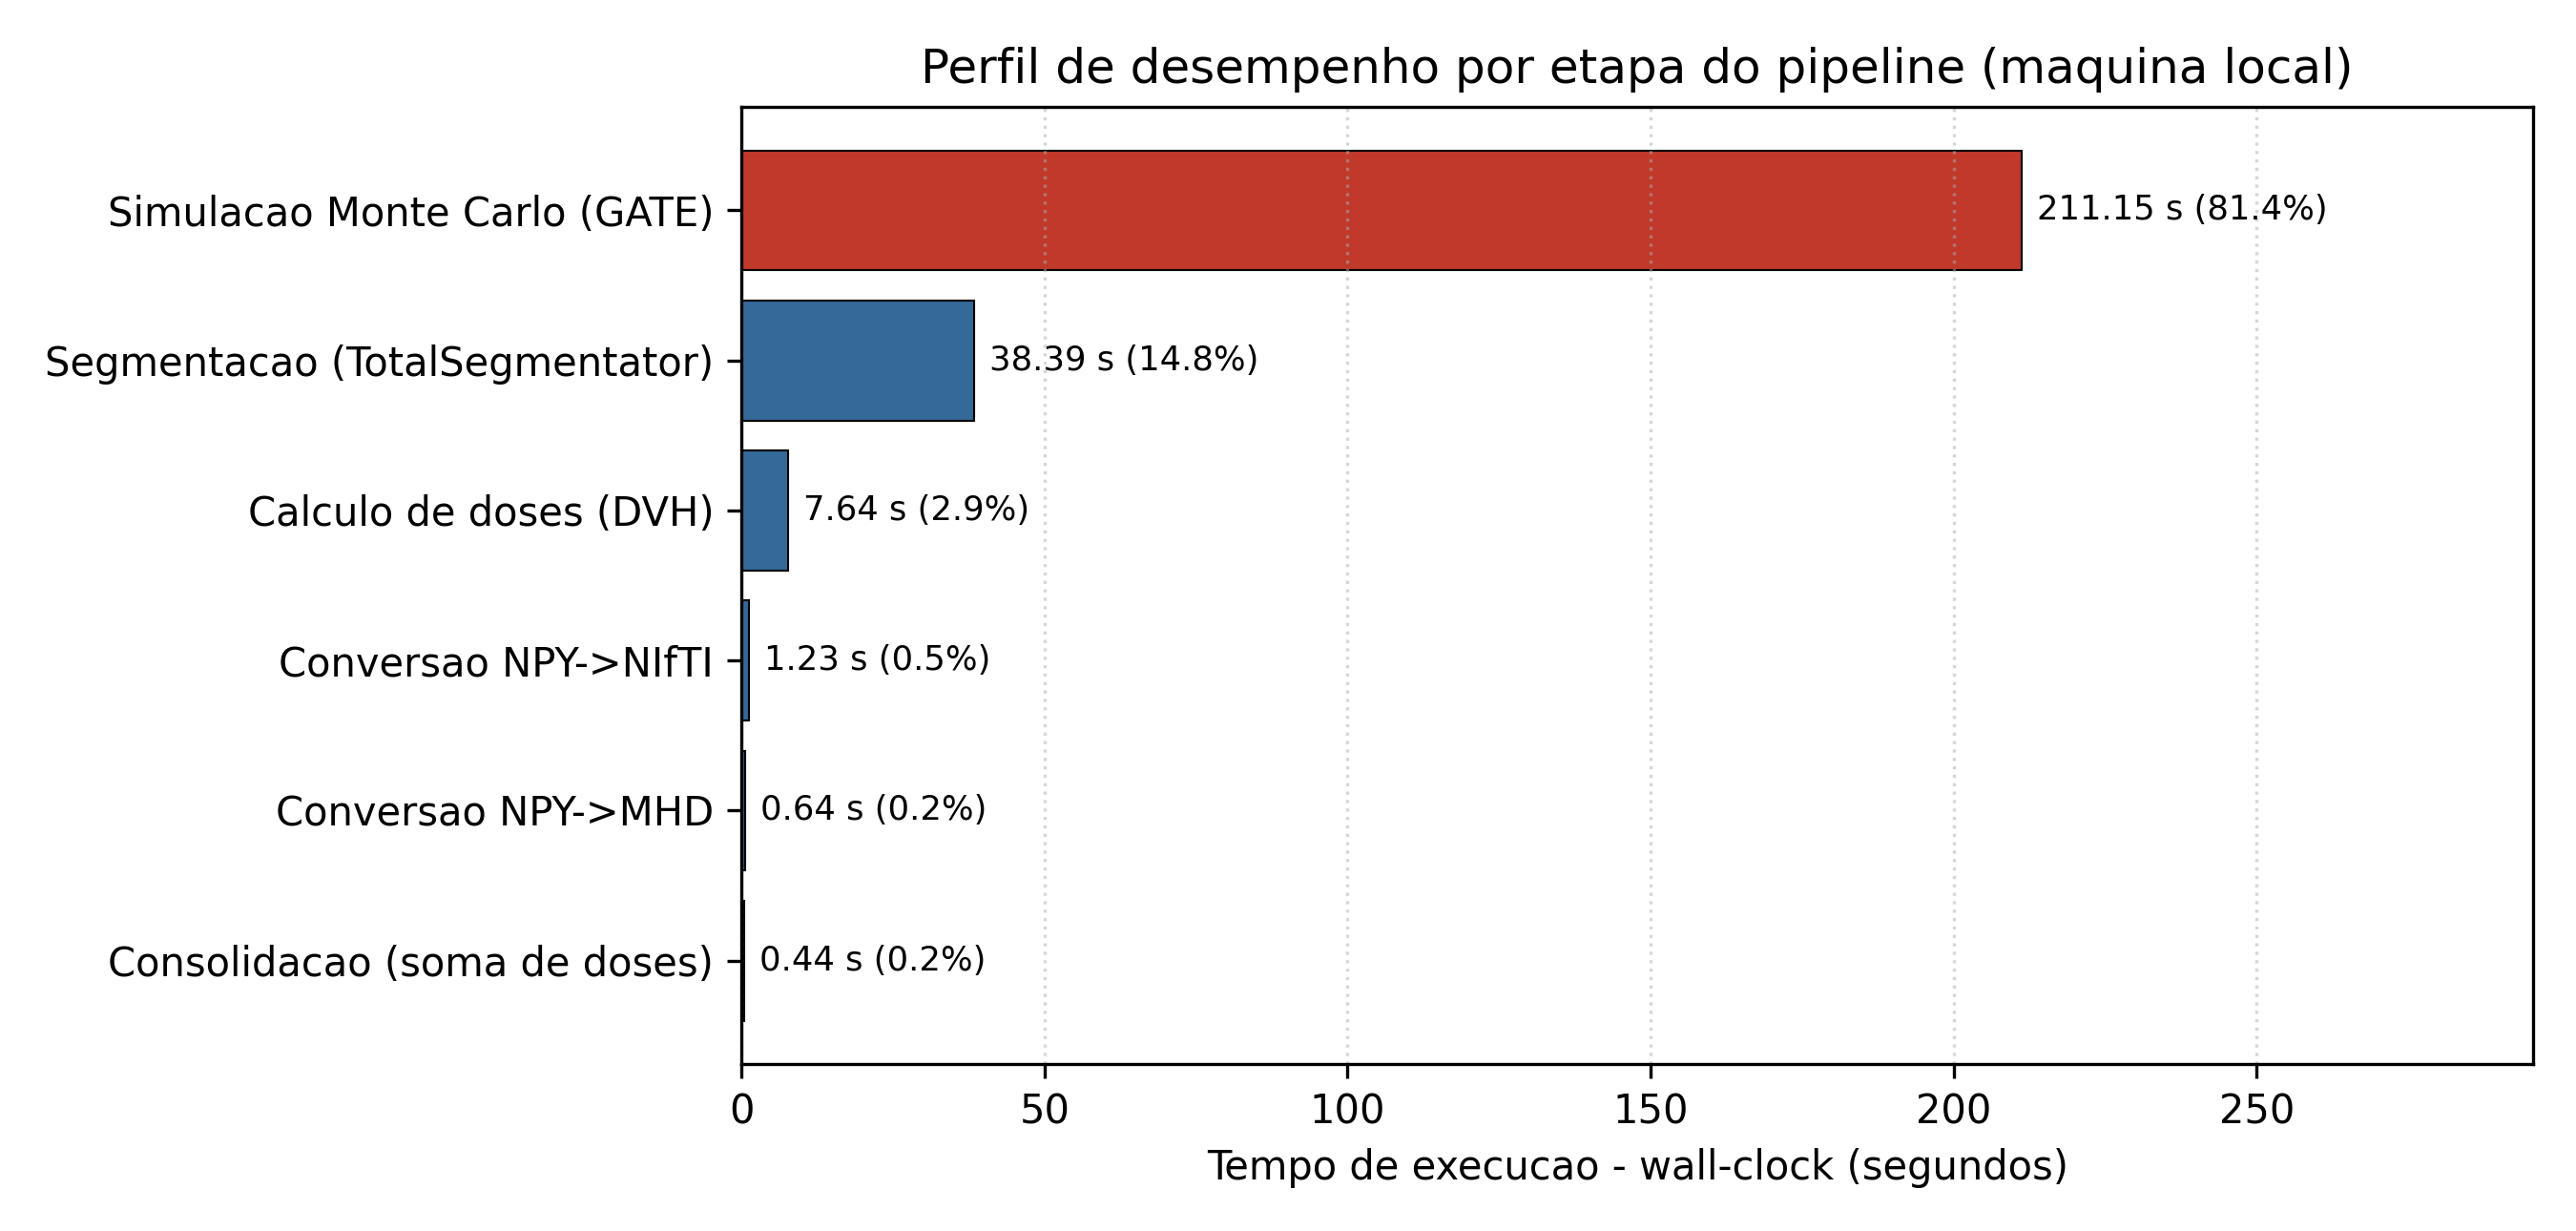
\includegraphics[width=0.95\textwidth]{fig1_perfil_etapas.png}
\caption{Perfil de tempo de execução (\textit{wall-clock}) por etapa do pipeline.
A simulação Monte Carlo (em destaque) responde por 81,4\% do tempo total.}
\label{fig:perfil}
\end{figure}

\subsection{Consumo de memória}
\label{sec:memoria}

Sob a ótica de memória (Figura~\ref{fig:memoria}), o pico de consumo ocorre na
segmentação com o TotalSegmentator (5,06~GB), coerente com a inferência da rede
nnU-Net, ainda assim muito inferior aos 503~GB disponíveis no servidor e
compatível com estações de trabalho modestas. O consumo de RAM é determinado
pelo tamanho do dado (volume $256^3$) e pelo modelo empregado, sendo portanto
independente da plataforma de execução; os valores da Tabela~\ref{tab:benchmarks}
valem, assim, como referência também para o ambiente HPC.

\begin{figure}[htbp]
\centering
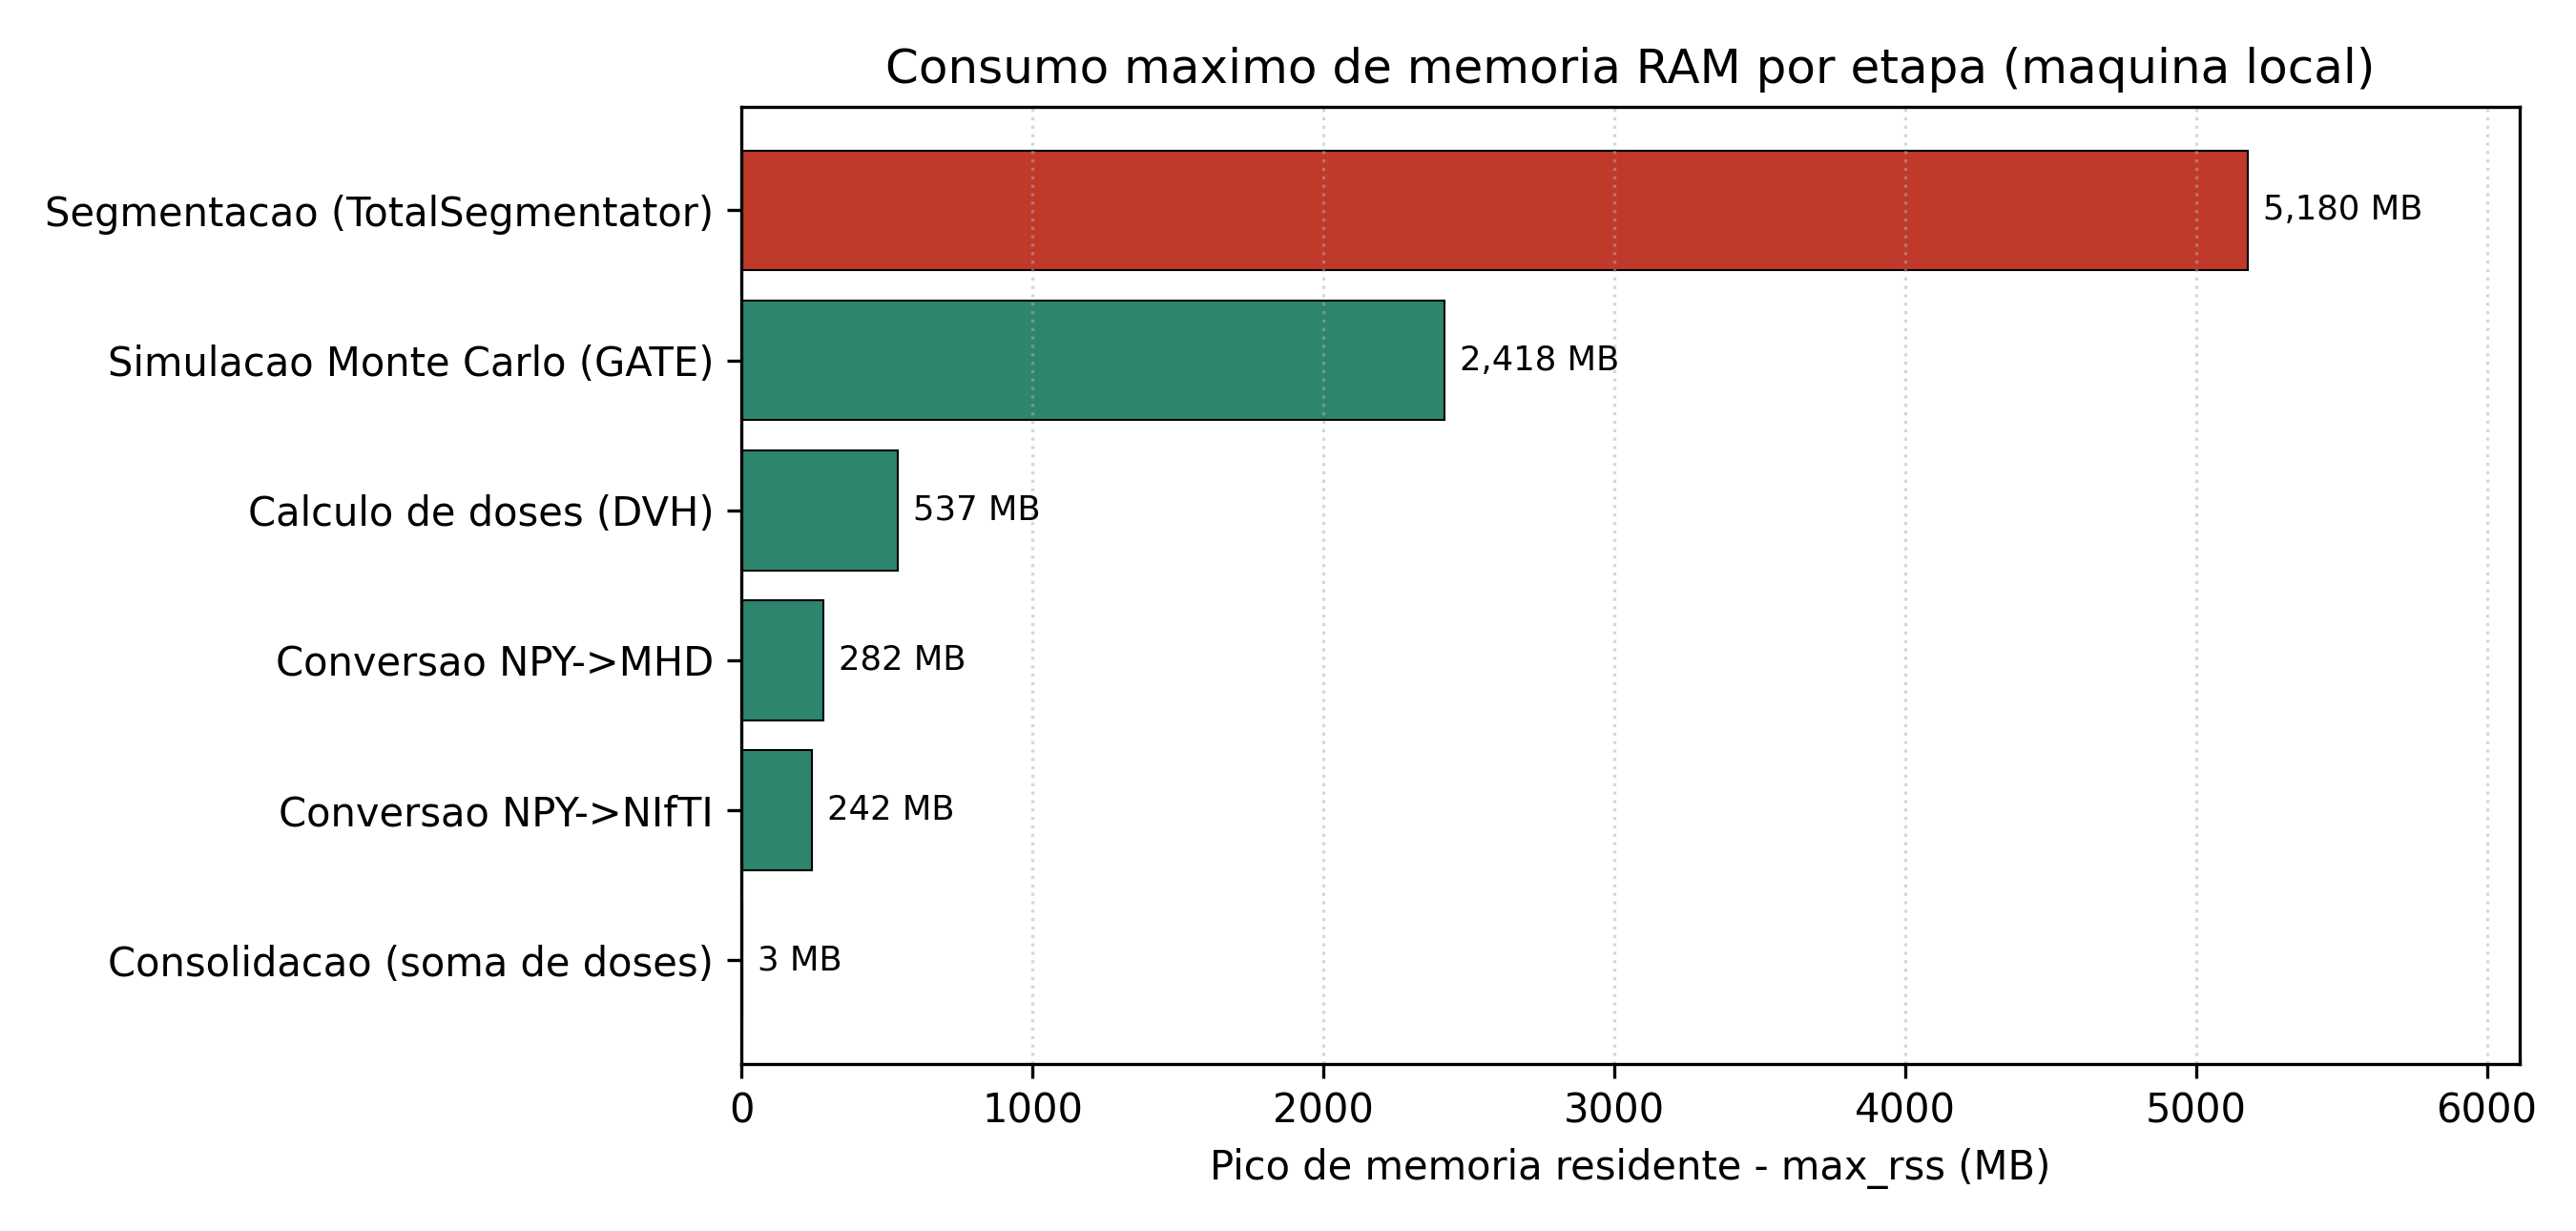
\includegraphics[width=0.95\textwidth]{fig2_memoria_etapas.png}
\caption{Pico de memória residente (\texttt{max\_rss}) por etapa do pipeline.
O maior consumo (5,06~GB) ocorre na segmentação.}
\label{fig:memoria}
\end{figure}

\subsection{Vazão por núcleo e escalabilidade da simulação}
\label{sec:escalabilidade}

Um resultado relevante emerge da comparação da vazão da simulação entre as duas
plataformas. Em execução \textit{single-thread}, a máquina local atinge
5.075~primárias/s, contra 2.119~primárias/s do servidor --- ou seja, o núcleo do
\textit{notebook} é cerca de \textbf{2,4 vezes mais rápido} por \textit{thread},
reflexo de sua maior frequência de operação e microarquitetura mais recente,
frente aos 2,1~GHz de base do processador de servidor. A vantagem do ambiente
HPC, portanto, \emph{não reside na velocidade por núcleo, mas na densidade de
paralelismo}.

A aquisição CBCT de $360^\circ$ possui paralelismo trivial: ela é decomposta em
\textbf{90 execuções independentes} (argumento \texttt{inicio} de 0 a 356, em
passos de 4), sem comunicação entre os processos. Cada execução --- doravante
denominada \textit{job} --- processa quatro projeções ($n=4$). A varredura
angular foi integrada ao Snakemake por meio de um \textit{wildcard} de ângulo,
de modo que a própria ferramenta gera os 90 \textit{jobs} e os agenda conforme o
número de núcleos informado na linha de comando (\texttt{snakemake --cores N}).
Definindo $t_{\text{job}}$ como o tempo de um \textit{job} e $p$ como o número de
processos concorrentes, o tempo total da aquisição é dado por

\begin{equation}
T(p) \;=\; \left\lceil \frac{N_{\text{jobs}}}{p} \right\rceil \cdot t_{\text{job}},
\qquad N_{\text{jobs}} = 90,
\label{eq:escalabilidade}
\end{equation}

\noindent
em que o operador teto ($\lceil\cdot\rceil$) contabiliza o número de ``levas''
de execução, dado que um \textit{job} é indivisível. Com
$t_{\text{job}} = 2{,}62$~h medido no HPC, a Figura~\ref{fig:escalabilidade}
mostra que a aquisição completa, se executada de forma estritamente serial,
exigiria cerca de 236~h ($\approx 9{,}8$ dias); distribuída pelos 48 núcleos
físicos do servidor, o tempo cai para cerca de 5,2~h; e com 90 a 96 processos
concorrentes (aproveitando o \textit{hyperthreading}), aproxima-se de cerca de
2,6~h --- limite imposto pela duração de um único \textit{job}. O comportamento
é praticamente linear, como esperado para uma carga sem dependências,
confirmando a escalabilidade da solução.

É importante destacar que o parâmetro $p$ da Equação~\ref{eq:escalabilidade}
corresponde exatamente ao número de núcleos solicitados ao Snakemake
(\texttt{--cores N}): \emph{não é necessário dispor de 90 núcleos} para executar
os 90 \textit{jobs}. Com $N$ núcleos, a ferramenta executa $N$ \textit{jobs}
simultaneamente e enfileira os demais, processando-os em $\lceil 90/N \rceil$
levas sucessivas, sem nunca exceder a capacidade da máquina. Esse controle
distingue a abordagem de um lançamento ingênuo de todos os processos de uma só
vez, que saturaria máquinas com poucos núcleos. Na prática, o limite efetivo de
$N$ é determinado tanto pelo número de núcleos quanto pela memória disponível,
uma vez que cada \textit{job} ocupa cerca de 2,4~GB de RAM
(Tabela~\ref{tab:benchmarks}); assim, a mesma definição de fluxo executa de forma
robusta tanto no servidor HPC ($N = 48$ a $96$) quanto em uma estação local
modesta ($N = 4$ a $6$), o que sustenta a portabilidade e a reprodutibilidade da
solução.

\begin{figure}[htbp]
\centering
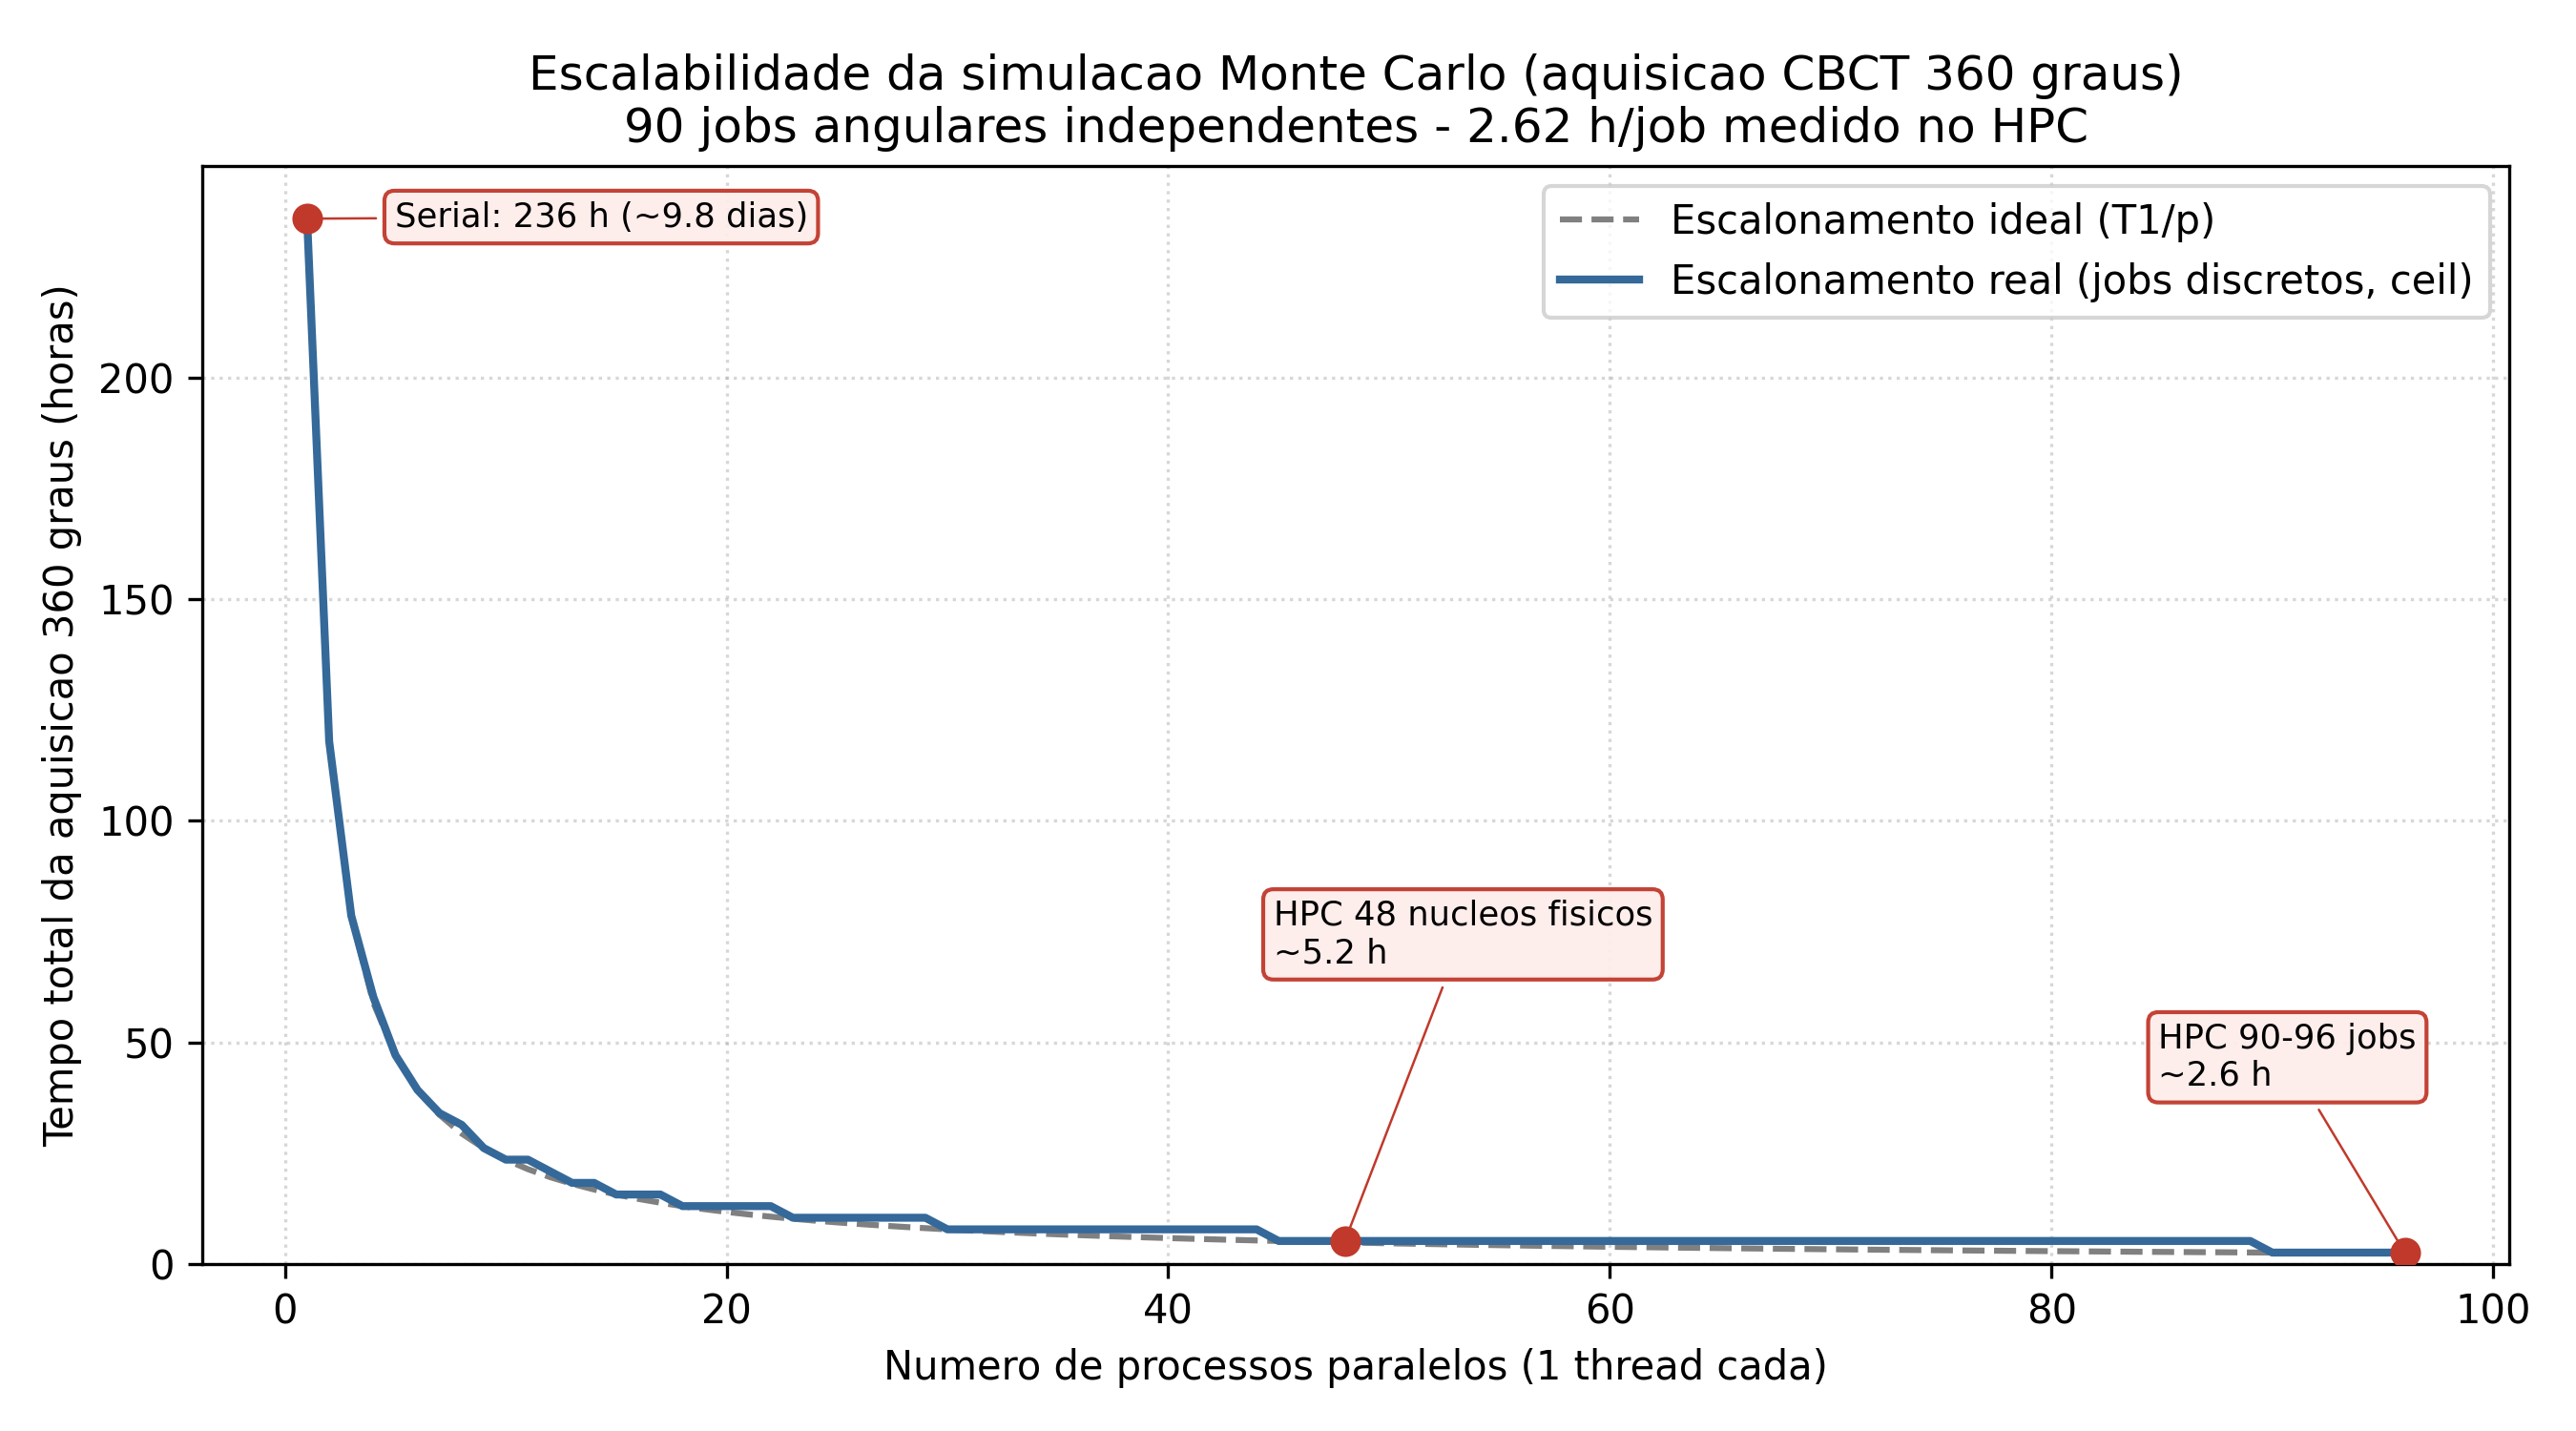
\includegraphics[width=0.95\textwidth]{fig3_escalabilidade.png}
\caption{Escalabilidade da simulação Monte Carlo para a aquisição de $360^\circ$.
Tempo total $T(p)$ (Equação~\ref{eq:escalabilidade}) em função do número de
processos concorrentes, com $t_{\text{job}} = 2{,}62$~h medido no HPC. A curva
tracejada indica o escalonamento ideal ($T_1/p$).}
\label{fig:escalabilidade}
\end{figure}

\subsection{Comparação entre plataformas}
\label{sec:comparacao}

A Figura~\ref{fig:comparacao} sintetiza o impacto prático da escolha de hardware
para a aquisição completa na qualidade definitiva ($5\times10^{6}$ primárias por
projeção). Os tempos de \textit{job} foram \emph{medidos} em ambas as máquinas:
59~min por \textit{job} no \textit{notebook} e 157~min ($2{,}62$~h) no servidor;
os tempos de aquisição completa decorrem da aplicação da
Equação~\ref{eq:escalabilidade} a esses valores medidos.

Confirma-se um resultado contraintuitivo: por \textit{job}, o \textit{notebook}
é \textbf{2,7 vezes mais rápido} que o servidor. Executada serialmente, a
aquisição completa levaria 88,5~h ($\approx 3{,}7$ dias) no \textit{notebook},
contra 236~h ($\approx 9{,}8$ dias) no servidor. Entretanto, os 10 núcleos do
\textit{notebook}, em um \textit{chip} de baixo consumo, não sustentam carga
total prolongada: mesmo no melhor caso teórico (12 \textit{jobs} simultâneos,
cerca de 7,9~h, desconsiderando o \textit{throttling} térmico) ele não alcança o
servidor. O HPC, ao distribuir os 90 \textit{jobs} por seus 48--96 núcleos com
\textit{clock} sustentado, conclui a aquisição em \textbf{cerca de 2,6~h},
viabilizando ainda \textbf{cinco vezes mais estatística} por projeção
($5\times10^{6}$ contra $1\times10^{6}$ primárias) dentro de um tempo prático.

\begin{figure}[htbp]
\centering
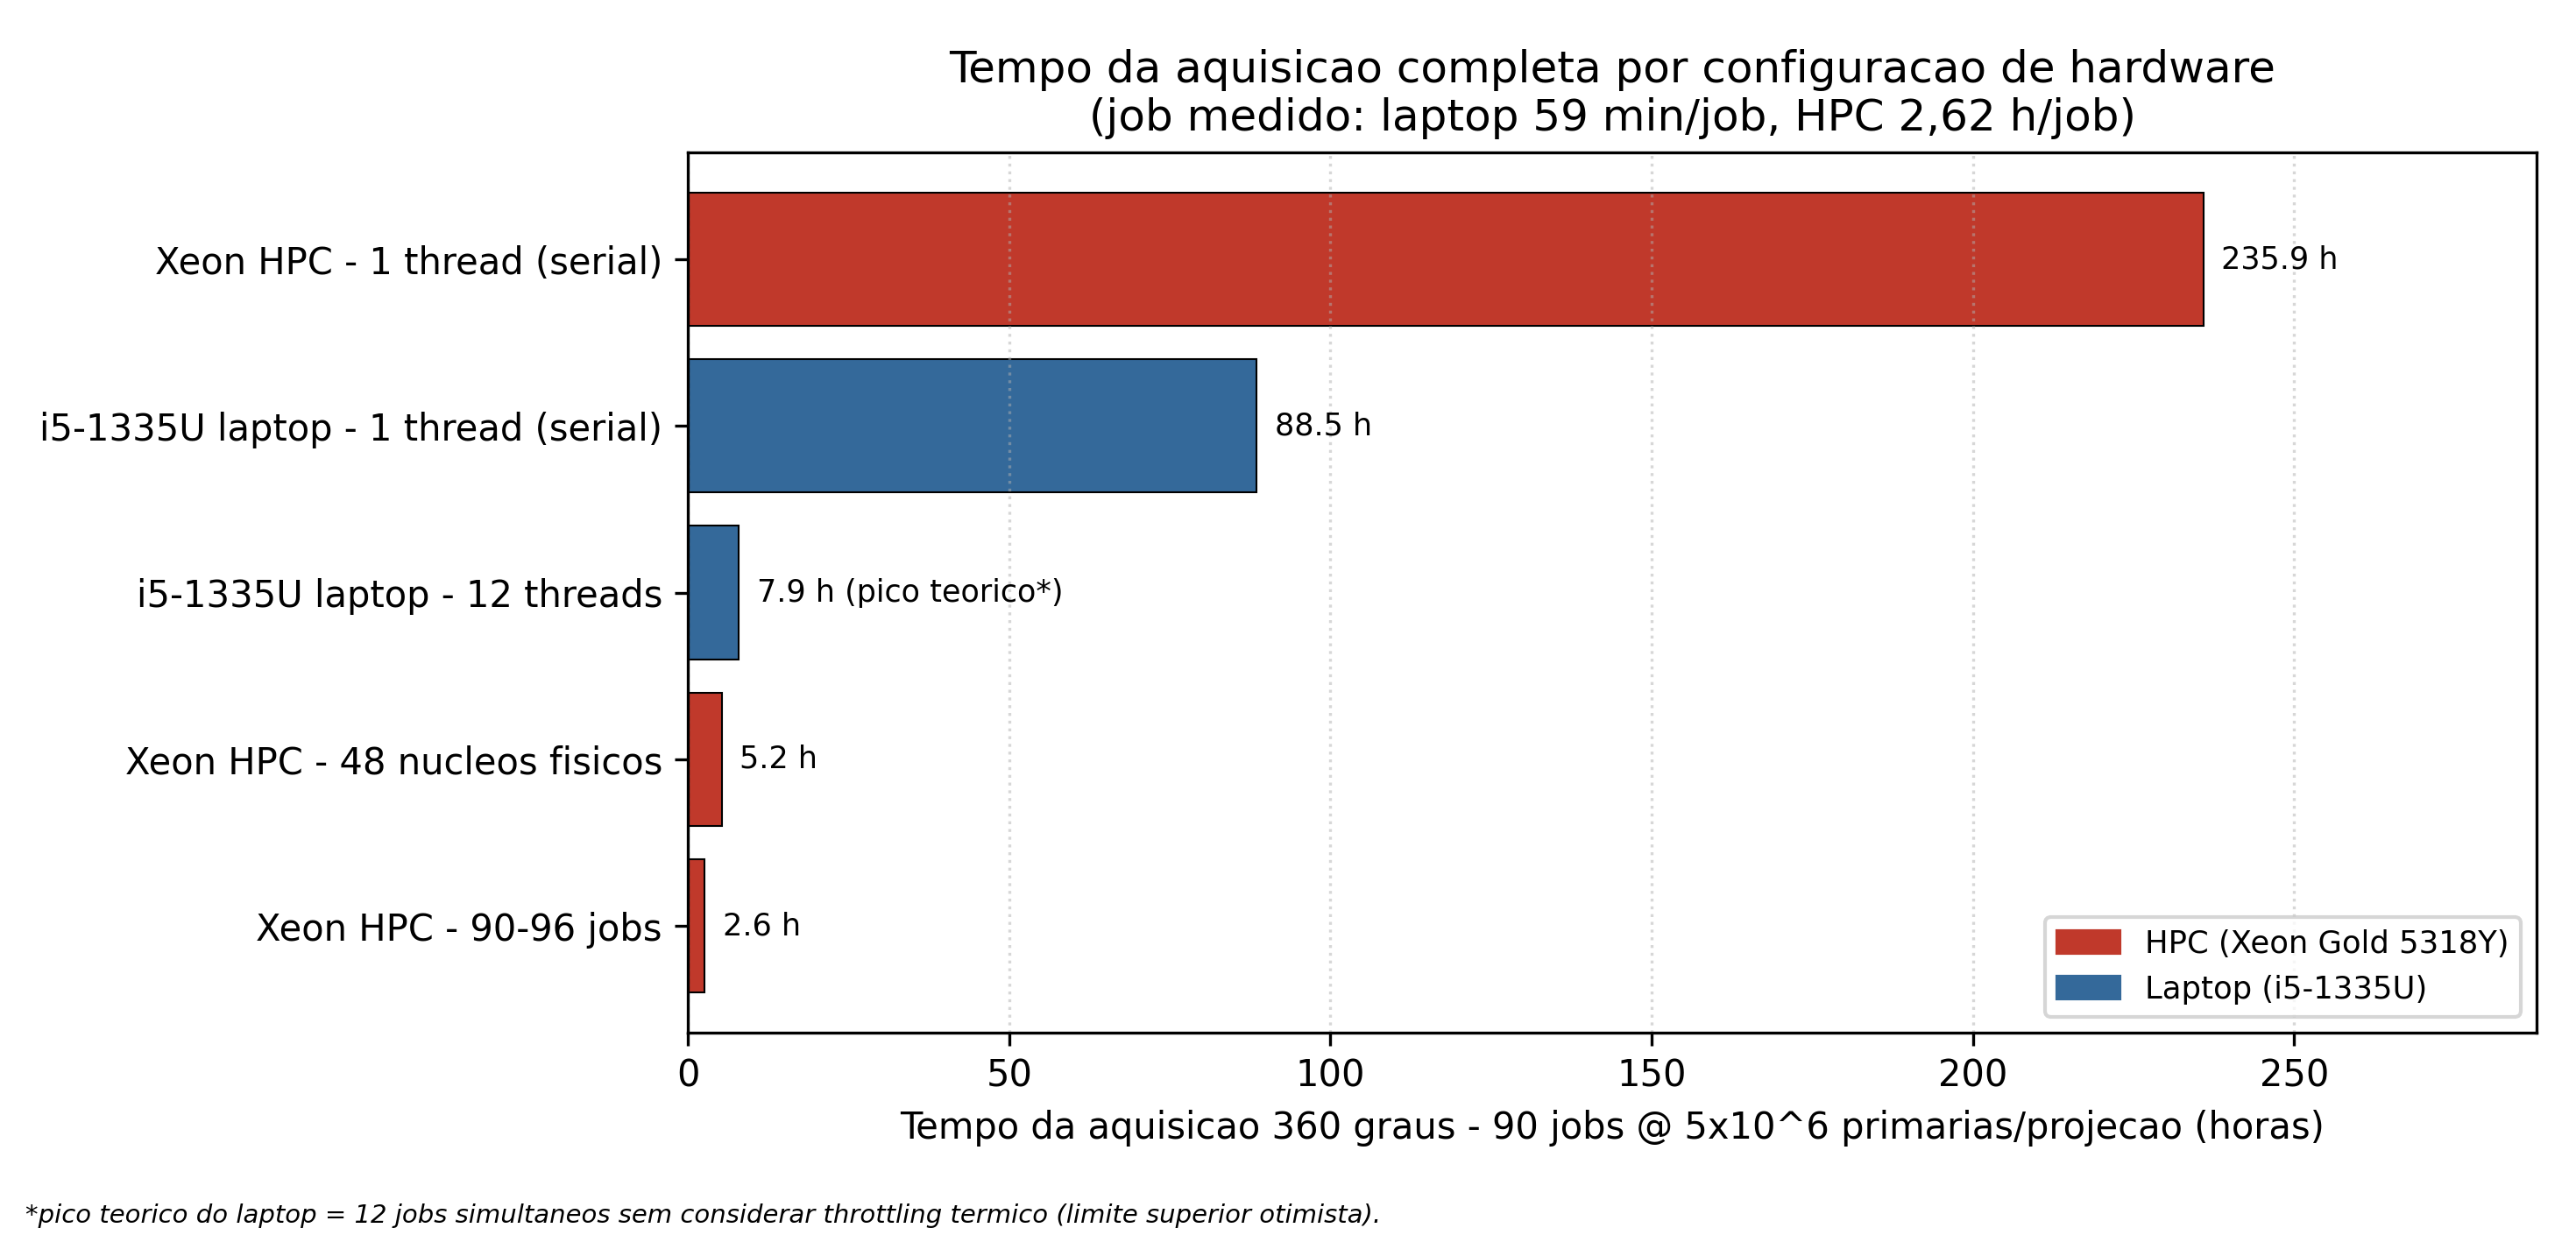
\includegraphics[width=0.97\textwidth]{fig4_comparacao_maquinas.png}
\caption{Tempo da aquisição completa de $360^\circ$ (90 \textit{jobs} a
$5\times10^{6}$ primárias/projeção) por configuração de hardware. Tempos de
\textit{job} medidos (laptop 59~min; HPC $2{,}62$~h); o tempo total decorre da
Equação~\ref{eq:escalabilidade}. A barra marcada com asterisco é um limite
superior otimista (não considera \textit{throttling} térmico do \textit{notebook}).}
\label{fig:comparacao}
\end{figure}

Conclui-se que o ganho de desempenho proporcionado pelo ambiente HPC decorre da
\emph{vazão agregada} e da \emph{robustez operacional} --- e não da velocidade
por núcleo --- justificando metodologicamente a produção dos resultados
definitivos no servidor, ao passo que a validação funcional integral do pipeline
foi conduzida na máquina local. Cabe ressaltar que todas as etapas foram
executadas com êxito em ambas as plataformas, atestando a portabilidade do
pipeline; a diferença reside exclusivamente no tempo de simulação, grandeza que
escala linearmente com o número de histórias e, por consequência, com a
qualidade estatística desejada.

% ============================================================================
%  NOTA DE INTEGRIDADE (NÃO COLAR NO TCC — apenas para você):
%  - Medido diretamente: tempos/RAM por etapa; pps (5075 e 2119); job de 59 min
%    (laptop) e 2,62 h (HPC).
%  - Derivado por linearidade (Eq. ref{eq:escalabilidade}): os tempos de
%    aquisicao completa (88,5 h; 7,9 h; 236 h; 5,2 h; 2,6 h) = job medido x 90.
%  - Unico valor "otimista": laptop 12 threads (7,9 h), pois ignora throttling.
%  - Confira no texto-base do metodo: HPC usou 5E6 prim/proj; local usou 1E6.
% ============================================================================
